\documentclass[letterpaper]{article} % DO NOT CHANGE THIS
\usepackage[submission]{aaai2027}  % DO NOT CHANGE THIS
\usepackage[hyphens]{url}  % DO NOT CHANGE THIS
\usepackage{graphicx} % DO NOT CHANGE THIS
\urlstyle{rm} % DO NOT CHANGE THIS
\def\UrlFont{\rm}  % DO NOT CHANGE THIS
\usepackage{natbib}  % DO NOT CHANGE THIS AND DO NOT ADD ANY OPTIONS TO IT
\usepackage{caption} % DO NOT CHANGE THIS AND DO NOT ADD ANY OPTIONS TO IT
\frenchspacing  % DO NOT CHANGE THIS

\usepackage{booktabs}
\usepackage{amsmath}
\usepackage{amssymb}

% Internal Chinese working draft only. The final English submission contains no
% CJK package or non-Roman text.
\usepackage{CJKutf8}
\makeatletter
\expandafter\let\csname ver@CJK.sty\endcsname\relax
\makeatother

\pdfinfo{
/TemplateVersion (2027.1)
}

\setcounter{secnumdepth}{0}

\title{\begin{CJK*}{UTF8}{gbsn}超越权重几何：以域条件功能谱追踪 On-Policy Distillation\end{CJK*}}
\author{Anonymous Submission}
\affiliations{}

\begin{document}
\maketitle
\begin{CJK*}{UTF8}{gbsn}

\begin{abstract}
权重几何描述参数在哪里变化，激活几何描述模型访问哪些方向，输出评测则记录完整网络最终产生了什么；三者之间仍缺少一个能够沿训练过程追踪局部计算的观察层。本文提出域条件功能谱：将线性模块的当前权重写入由指定输入域激活二阶矩定义的白化坐标，使其奇异谱直接对应本层输出能量，并具有精确的最优低秩输出误差解释。我们用该谱比较两种模型上的 OPD、SFT 与离线蒸馏轨迹，并通过 sequence exposure、rollout refresh 和 matched-support 对照收紧解释。双模型严格共同网格显示，该功能坐标保留了纯激活谱与 source-principal 权重位置不能单独提供的轨迹和输出移动信息。OPD 在共同早期窗口进入更深的跨域功能压缩状态，持续刷新 current-student support 是这一轨迹的重要组织因素。相对功能压缩还追踪推理、格式、答案和终止区域的无符号输出移动，而相近的功能路径仍可产生不同读出。域条件功能谱由此提供了裸权重与最终行为之间的功能观察层，而不是端到端行为的充分统计量。
\end{abstract}

\section{引言}

大模型后训练不是从初始模型到终点模型的一次跳跃。相邻 checkpoint 之间可能出现 OOD 能力下降与恢复、生成长度突变、终止失败以及严格格式漂移；只比较起点和终点会丢失这些暂态 \citep{ren2026rethinking,jin2025rlheals}。这一问题在 on-policy distillation（OPD）中尤其突出：模型用当前学生生成 rollout，再在这些前缀上接受教师分布监督，因此训练支持本身会随学生共同演化 \citep{agarwal2024opd,li2026rethinkingopd}。

现有分析分别观察三个层次。权重几何用更新范数、秩、奇异子空间和 source-principal 位置描述参数如何改变 \citep{shuttleworth2024lora,zhu2025path,yu2026dense,shen2026geometryopd}；激活几何用有效秩、participation ratio、各向异性和 CKA 描述输入表示访问了哪些方向 \citep{liu2026collapse}；KL、NLL 和下游任务则观察完整网络的最终输出。前两者各自遗漏了输入访问或权重对输入方向的作用，后者又把所有层和模块压缩成最终读出。它们都没有直接回答：当前权重在某个输入域上实际使用了哪些功能方向，这些方向又如何随训练改变？

我们提出域条件功能谱来填补这一观察层。对 checkpoint $t$ 的线性模块权重 $W_t$，以及输入域 $D$ 上模块输入激活的二阶矩平方根 $S_{D,t}$，我们分析
\begin{equation}
A_{D,t}=W_tS_{D,t}.
\label{eq:intro-state}
\end{equation}
$A_{D,t}$ 不是把权重特征与激活特征事后拼接，而是同一个权重映射在域条件白化输入坐标中的矩阵表示。其奇异值平方就是模块输出二阶矩的特征值；截断该谱等价于在域 $D$ 上最小化期望本层输出误差。由此得到的功能秩回答：为了保留当前模块在该域上的主要输出能量，至少需要多少方向？

我们把这一静态的局部近似空间转化为 checkpoint-wise 观察方法，并围绕 sequence support 构造控制链。OPD 与 off-KD 共享 forward KL、但使用 current-student 与 frozen-teacher 序列；$\alpha=.5$ 改变 current-self exposure；frozenSelf0-KD 则固定 step-0 student rollout，只移除持续 refresh；off-KD 与 seqKD 进一步保持序列完全相同、只改变 soft 与 hard target。本文的主要发现是：
\begin{itemize}
    \item 域条件功能谱给出具有精确本层输出误差含义的内部状态量，并在双模型严格共同网格中保留纯激活谱和 source-principal 权重位置不能单独提供的轨迹信息。
    \item 在 Qwen3-4B-Base 与 Llama-3.2-3B 的共同早期窗口，OPD 均进入更深的跨域功能压缩状态；exposure 与 frozen-self 对照进一步表明 current-support refresh 组织了这一轨迹。
    \item 相对功能压缩与推理、格式、答案和终止区域的无符号输出移动同步，但区域分配、signed readout 和自由生成行为具有模型与训练目标依赖性，显示功能模式预算与最终读出的分离。
\end{itemize}

\section{相关工作}

\subsection{On-Policy 蒸馏与后训练轨迹}

经典知识蒸馏在固定数据上匹配教师软目标 \citep{hinton2015distilling}；GKD/OPD 把教师反馈施加到当前学生访问的状态，以减小训练与推理支持之间的不匹配 \citep{agarwal2024opd}。后续工作讨论 teacher--student gap、cold start、支持重叠和监督粒度 \citep{li2026rethinkingopd,song2026surveyopd,yang2026oprd}。本文不提出新的训练目标，而是测量 sequence producer、support refresh 与 target 如何组织逐 checkpoint 的内部功能轨迹。

\subsection{权重、激活与功能空间}

权重空间工作测量更新尺度、谱集中、principal-coordinate mask、source-principal 投影以及奇异子空间旋转 \citep{zhu2025path,jin2025rlheals,yu2026dense}。这些量可以回答更新写入哪里，却不随输入域改变。纯激活谱与表示相似性描述 hidden states 如何铺开或重组，但不知道当前权重如何放大、压低或旋转这些方向。本文的 $W_tS_{D,t}$ 以激活定义输入度量，再在该度量中观察完整权重映射，因而位于裸权重与最终输出之间，而不是二者的替代。

\subsection{Activation-Aware 低秩近似}

裸权重 SVD 在隐藏坐标的 Euclidean 度量下最小化 Frobenius 误差，对频繁访问和几乎不访问的输入方向一视同仁。Fisher-weighted SVD 用参数敏感性近似重加权这一目标 \citep{hsu2022fisherweighted}；ASVD 与 SVD-LLM 使用校准激活改进静态权重分解 \citep{yuan2024asvd,wang2025svdllm}。本文沿用 activation-aware 分解的关键等式，但改变用途：我们不压缩模型，而是在每个 checkpoint 和输入域上重新测量当前功能状态。与全网络 Fisher、Jacobian 或 Taylor 诊断相比 \citep{amari1998natural,martens2015kfac,saadi2025flex}，该空间只处理单层线性二阶问题，却不需要梯度或全网络近似，并在这个局部问题上保持精确。

\section{域条件功能谱}

\subsection{白化坐标中的同一权重映射}

固定 checkpoint、输入域和线性模块。令 $h$ 为模块输入，
\begin{equation}
\Sigma_{D,t}=\mathbb E_{h\sim D}[hh^\top],
\qquad
S_{D,t}S_{D,t}^{\top}=\Sigma_{D,t}.
\label{eq:second-moment}
\end{equation}
若 $\Sigma_{D,t}$ 满秩，取 $z=S_{D,t}^{-1}h$；若其秩亏，则在支撑空间取 $z=S_{D,t}^{\dagger}h$。两种情况下都有
\begin{equation}
h=S_{D,t}z,\qquad \mathbb E[zz^\top]=I,\qquad
W_th=(W_tS_{D,t})z
\label{eq:whitened-map}
\end{equation}
（最后一个恒等式中的 $I$ 限定在支撑空间）。因此 $A_{D,t}=W_tS_{D,t}$ 表示的仍是 $W_t$，只是输入坐标已经按该域实际访问的尺度和相关性白化。裸权重中的大奇异值不一定在域输入上产生大输出；功能谱消除了这种坐标尺度错配。

该表示还直接连接本层输出。其左 Gram 矩阵为
\begin{equation}
A_{D,t}A_{D,t}^{\top}
=W_t\Sigma_{D,t}W_t^\top
=\mathbb E[(W_th)(W_th)^\top].
\label{eq:output-energy}
\end{equation}
所以 $\sigma_i^2(A_{D,t})$ 是模块输出二阶矩的第 $i$ 个特征值。裸权重谱正是 $S=I$ 的特殊情形：
\begin{equation}
\mathbb E_{z:\,\mathbb E[zz^\top]=I}
\|(W_t-\widetilde W)z\|_2^2
=\|W_t-\widetilde W\|_F^2.
\end{equation}
它隐含地把所有输入方向视为互不相关、单位尺度且同等重要；$S_{D,t}$ 则用模型在域 $D$ 上实际经历的输入度量替换这一假设。进一步地，对任意候选近似 $\widetilde W$，
\begin{equation}
\mathbb E\|W_th-\widetilde Wh\|_2^2
=\|(W_t-\widetilde W)S_{D,t}\|_F^2.
\label{eq:output-error}
\end{equation}
写 $A_{D,t}=\sum_i\sigma_i u_iv_i^\top$，保留最大的 $k$ 个方向得到
$A_{D,t}^{(k)}=\sum_{i\le k}\sigma_i u_iv_i^\top$。正交性给出
\begin{equation}
\|A_{D,t}-A_{D,t}^{(k)}\|_F^2=\sum_{i>k}\sigma_i^2,
\end{equation}
而 Eckart--Young 定理保证任意 rank-$k$ 矩阵 $B$ 的误差都不小于该尾部能量 \citep{eckart1936approximation}。结合式~\eqref{eq:output-error}，丢弃较小功能奇异方向正好最小化域条件期望本层输出误差。完整证明、秩亏情形、坐标不变性与扰动界见 Supplementary Secs.~A.1--A.5。

\subsection{功能秩与轨迹量}

令 $\sigma_1\ge\cdots\ge\sigma_q$ 为 $A_{D,t}$ 的奇异值。允许丢弃尾部能量比例 $\varepsilon$ 时，定义
\begin{equation}
r_\varepsilon(A_{D,t})
=\min\left\{r:
\frac{\sum_{i>r}\sigma_i^2}{\sum_i\sigma_i^2}\le\varepsilon
\right\}.
\label{eq:functional-rank}
\end{equation}
$r_\varepsilon$ 越小，表示主要本层输出能量集中在越少的功能模式。主结果使用 $\varepsilon=.05$，并以其他阈值、stable rank 和 entropy effective rank 检查离散阈值敏感性。

七类 projection 的矩阵形状和基线功能秩不同；直接平均方向数变化会让初始秩较大的模块自然占据更大权重。为描述一个典型 projection 相对自身模式预算的重组程度，主轨先在
\begin{equation}
\mathcal M_5=\{v,o,\mathrm{gate},\mathrm{up},\mathrm{down}\}
\end{equation}
中逐模块相对各自基线归一化，再等权平均：
\begin{equation}
c_{\varepsilon,D,a,t}^{(5)}
=\frac{1}{5}\sum_{j\in\mathcal M_5}
\frac{r_{\varepsilon,D,a,0,j}-r_{\varepsilon,D,a,t,j}}
{r_{\varepsilon,D,a,0,j}}.
\label{eq:relative-contraction}
\end{equation}
这里的 equal-5 是投影类型的相对变化摘要，不是功能能量归因。q/k 共同决定 attention routing，且其较低基线功能秩使少量方向变化具有较高杠杆；逐模块审计还显示其训练设置排序与其余五类不同。因此我们独立报告 q/k 和 equal-7 敏感性。全部七模块结果与 paired equal-5/equal-7 比较见 Supplementary Sec.~C.2。

\section{实验设计}

\subsection{模型、训练设置与输入域}

主实验包含 Qwen3-4B-Base 与 Llama-3.2-3B 两个学生模型，均采用 rank-32 LoRA 后训练 \citep{hu2022lora,qwen2025technical,meta2024llama32}。OPD 使用 current-student rollout 并匹配 dense teacher distribution \citep{verl2025opd}；SFT 使用外部参考推理序列和 hard next-token supervision。二者同时改变 sequence producer、support 与目标，因而后续对照按问题逐步收紧。off-KD 保持 teacher forward KL、但将序列换为冻结 teacher rollout，用于定位 sequence source；Qwen 的 $\alpha=.5$ 在同一目标下改变 current-student exposure；Llama frozenSelf0-KD 保留 step-0 student 生成的序列来源、但永久冻结 rollout，用于隔离持续 refresh；seqKD 则与 off-KD 共享完全相同的 teacher sequences、顺序、步数和 LoRA 配置，只把 dense target 换成 hard next-token target。

四个冻结输入域承担不同角色。General 使用 WikiText 文本切片，提供非数学、非指令型锚点 \citep{merity2017pointer}；held-out math 使用与训练和 MATH500 排除重叠的 Hendrycks MATH 题面，测量同任务族的外部分布 \citep{hendrycks2021math}；MMLU-Pro 使用冻结的问题与选项文本，覆盖多学科知识和推理 \citep{wang2024mmlupro}；IFEval 只使用冻结的约束指令 prompt，观察格式和指令域上的输入条件状态 \citep{zhou2023ifeval}。它们用于采集激活，不等同于相应 benchmark 的行为分数。Qwen 主层为 L18，Llama 主层为 L14，均按架构中点预先选定；样本、去重、mask 及浅深层重复见 Supplementary Secs.~B.2 与 C.3。跨设置比较只使用严格共同 checkpoint；共同早期窗口为 step 20、40 和 80，轨迹面积积分至 step 320。

\subsection{数值与统计协议}

功能谱从序列化 BF16 deployed merged checkpoint 读取，两条轨均使用 BF16 forward、FP32 构造 $WS$，并以 FP64 完成对称特征分解与 SVD；Llama 在 FP32 累积 Gram 后转入 FP64 分解，而 Qwen 的审计轨以 FP64 记录 Gram/whitening。我们先在每个样本的有效 token/window 内归一化，再对样本等权，避免长文本自动获得更大权重。独立数值轨的 $r_{.05}$ 在共同单元上达到 Spearman $.9966$、MAE $.00050$。完整样本数、mask、tie rule、dtype parity 和 teacher top-32 retained-mass 审计见 Supplementary Secs.~B.2--B.4。

probe、domain、module 和 checkpoint 是同一条训练轨迹上的相关测量，而不是独立训练重复。训练设置内 Spearman 描述随训练累积的单调关系；checkpoint-demeaning 在同一 model--domain--checkpoint 内减去四设置均值，询问相同训练阶段的横向关系；样本外模型按 checkpoint group 留一，标准化和 ridge 强度只在训练 folds 内拟合。

\subsection{区域输出与比较坐标}

我们在固定参考序列上 teacher forcing，计算 base 到 checkpoint 的 full-vocabulary
$D_{\mathrm{KL}}(p_0\Vert p_t)$。MMLU-Pro 划分为 prompt $P$、正确标签前的格式 token $F$、表示正确选项标签的区域 $A$ 和 termination $T$；MATH500 划分为 prompt $P$、固定参考解答中 boxed answer 之前的推理 $C$、token-clean 完整 boxed-answer span $B$ 和 termination $T$。主 KL 区域为 MMLU-Pro 的 $F/A/T$ 与 MATH500 的 $C/B/T$；先在每题区域内平均，再对样本 macro 平均。signed NLL 保留 reference-token likelihood 改善或恶化的方向。完整 token mask、边界规则和旧整段 reference-stream 敏感性见 Supplementary Secs.~B.2 与 D.1。

比较坐标覆盖激活、更新位置与权重子空间。纯激活代表量为 centered covariance 的 entropy effective rank \citep{liu2026collapse}
\begin{equation}
\mathrm{ER}=\exp\!\left(-\sum_iq_i\log q_i\right),\qquad
q_i=\lambda_i/\sum_j\lambda_j.
\end{equation}
TPNT 统计更新坐标在 source rank-$k$ principal mask 中相对同密度随机 mask 的覆盖富集 \citep{yu2026dense,zhu2025path}；PABS 是 source 与 checkpoint 的 top-$k$ 左右奇异子空间 principal-angle cosine 的平均，越接近 1 表示旋转越小 \citep{jin2025rlheals}。完整 activation suite $A$ 还包括 PR、top-1/8/32 share、raw/centered anisotropy 与 step-0 CKA。纯权重强基线 \citep{yu2026dense} 为 source-principal 联合投影
\begin{equation}
p_k=\frac{\|U_k^\top\Delta W V_k\|_F^2}{\|\Delta W\|_F^2},
\qquad k\in\{4,8,16,32\},
\label{eq:pk}
\end{equation}
其中 $U_k,V_k$ 来自 source 权重的 top-$k$ 奇异子空间，$\Delta W$ 使用 deployed merged checkpoint 减 base。NSS 和其余原生指标见 Supplementary Sec.~B.4。比较均在共同 cells、共同模块集合和相同 checkpoint-held-out folds 上完成。

\section{结果}

\begin{figure*}[!t]
\centering
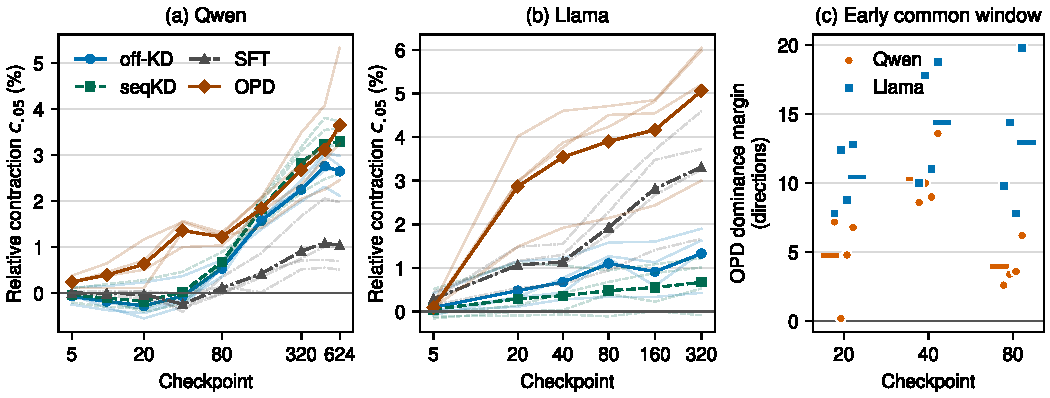
\includegraphics[width=\textwidth]{figures/fig1_main_trajectories.pdf}
\caption{纯激活、纯权重与功能轨迹。上行为 Qwen，下行为 Llama；各列依次为 activation ER、TPNT 相对 null 的 excess lift、PABS drift $10^4(1-\mathrm{PABS})$ 和 equal-5 相对功能压缩。四列量纲不同，原始纵轴幅度不可跨列比较；曲线仅连接实际 checkpoint。功能谱呈现了前三类坐标未共同复现的训练设置分离。}
\label{fig:main}
\end{figure*}

\begin{table*}[!t]
\centering
\small
\setlength{\tabcolsep}{5pt}
\begin{tabular}{lccc}
\toprule
模型 & Activation suite $A$ & Functional $C_5$ & Weight $P_{k,5}$ \\
\midrule
Llama & .556 & \textbf{.743} & .688 \\
Qwen & .595 & \textbf{.708} & .521 \\
\bottomrule
\end{tabular}
\caption{严格共同网格上的 OPD 识别（checkpoint-held-out AUC）。每个模型使用 64 个共同状态、相同 equal-5 模块和 folds。$A$ 是包含 ER、PR、top-1/8/32 share、raw/centered anisotropy 与 step-0 CKA 的八维纯激活特征组，不是图~\ref{fig:main} 中的 ER 单项。}
\label{tab:identification}
\end{table*}

\begin{table*}[!t]
\centering
\small
\setlength{\tabcolsep}{4pt}
\begin{tabular}{lrrrrr}
\toprule
模型 & $M_{\min}^{\mathrm{early}}$ & OPD NCD & SFT NCD & off-KD NCD & seqKD NCD \\
\midrule
Qwen & .200 & \textbf{50.423} & 9.554 & 31.017 & 37.793 \\
Llama & 7.800 & \textbf{77.594} & 39.683 & 17.518 & 11.093 \\
\bottomrule
\end{tabular}
\caption{共同早期排序与全轨迹压缩剂量。$M_{\min}^{\mathrm{early}}$ 是四核心域和共同早期 checkpoint 上的最小 OPD 连续边际（directions）；正值排除该范围内的排序反转。NCD 在 $\log(1+t)$ 上积分至 $T=320$（directions$\times$log-step），衡量压缩深度与持续时间。两列尺度不可直接比较。}
\label{tab:ncd}
\end{table*}

\begin{figure*}[!t]
\centering
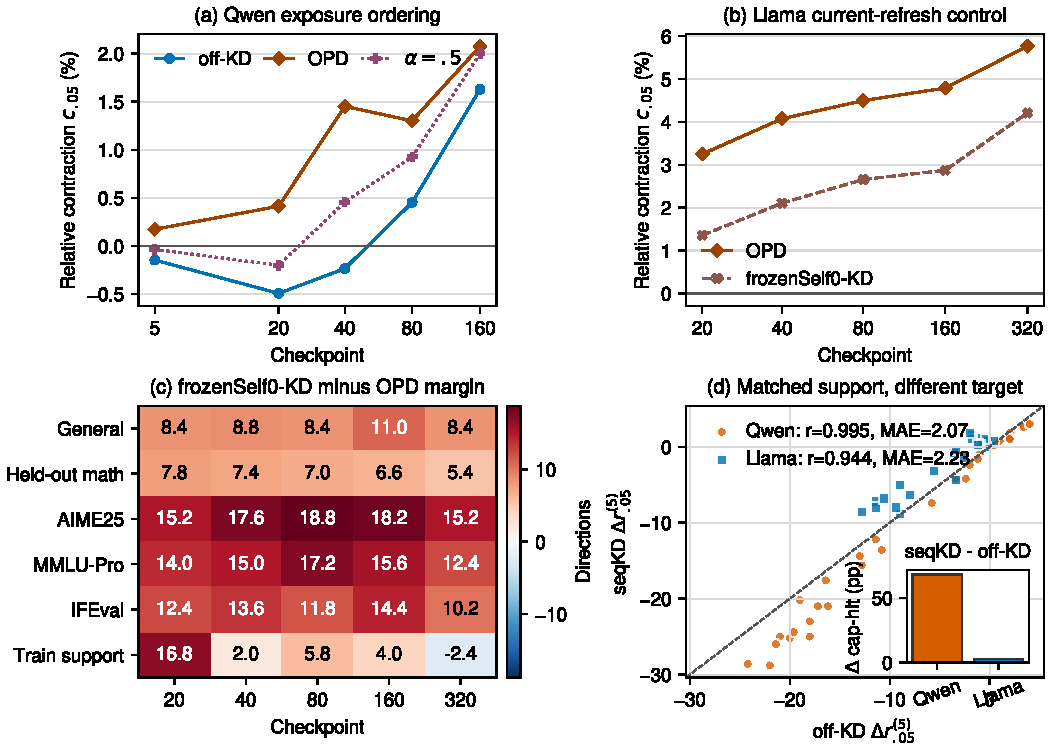
\includegraphics[width=\textwidth]{figures/fig2_support_controls.pdf}
\caption{Sequence exposure 与 refresh 对照。（a）Qwen $\alpha=.5$ 相对 off-KD 和 OPD 的有序轨迹。（b）Llama OPD 与 frozenSelf0-KD 在五个固定外部域上的等域平均绝对轨迹。（c）对应的逐域配对边际；正值表示持续刷新的 OPD 更压缩，粗黑线为外部域均值。图例中的 Math、AIME、MMLU 和 Mean 分别表示 held-out math、AIME25、MMLU-Pro 和五域均值。}
\label{fig:controls}
\end{figure*}

\begin{table*}[!t]
\centering
\small
\setlength{\tabcolsep}{2.7pt}
\textbf{A. off-KD 与 seqKD 的逐域 equal-5 路径一致性（Pearson $r$/MAE directions）}\\[2pt]
\begin{tabular}{lccccc}
\toprule
模型 & General & Math & MMLU-Pro & IFEval & Pooled \\
\midrule
Qwen & .995/1.13 & .996/2.67 & .998/2.18 & .999/2.29 & .995/2.07 \\
Llama & -.771/2.53 & .971/1.73 & .968/2.23 & .824/2.40 & .944/2.23 \\
\bottomrule
\end{tabular}

\vspace{4pt}
\textbf{B. 匹配训练设置的终点行为（\%）}\\[2pt]
\begin{tabular}{llrrrrrrr}
\toprule
模型 & 设置 & \multicolumn{2}{c}{MATH500} & \multicolumn{3}{c}{MMLU-Pro} & \multicolumn{2}{c}{IFEval} \\
\cmidrule(lr){3-4}\cmidrule(lr){5-7}\cmidrule(lr){8-9}
 & & Acc. & Cap & Strict & Flex. & Extract & Prompt & Instr. \\
\midrule
Qwen & off-KD & 79.4 & 4.8 & 35.4 & 57.1 & 47.3 & 23.1 & 36.5 \\
 & seqKD & 72.4 & 73.0 & 30.6 & 58.1 & 54.1 & 24.4 & 39.3 \\
Llama & off-KD & 8.2 & 91.8 & 14.2 & 16.4 & 50.3 & 19.6 & 33.2 \\
 & seqKD & 10.2 & 94.6 & 13.1 & 15.4 & 51.6 & 19.2 & 31.5 \\
\bottomrule
\end{tabular}
\caption{Matched-support 的功能路径与行为读出。A 使用完全匹配的非零 checkpoint；MAE 是逐 checkpoint 的方向差。B 使用 Qwen step 624 与 Llama step 320；Cap 为 generation-cap hit，Extract 为 extraction failure，Prompt/Instr. 为 IFEval prompt/instruction strict。}
\label{tab:support-readout}
\end{table*}

\begin{figure*}[!t]
\centering
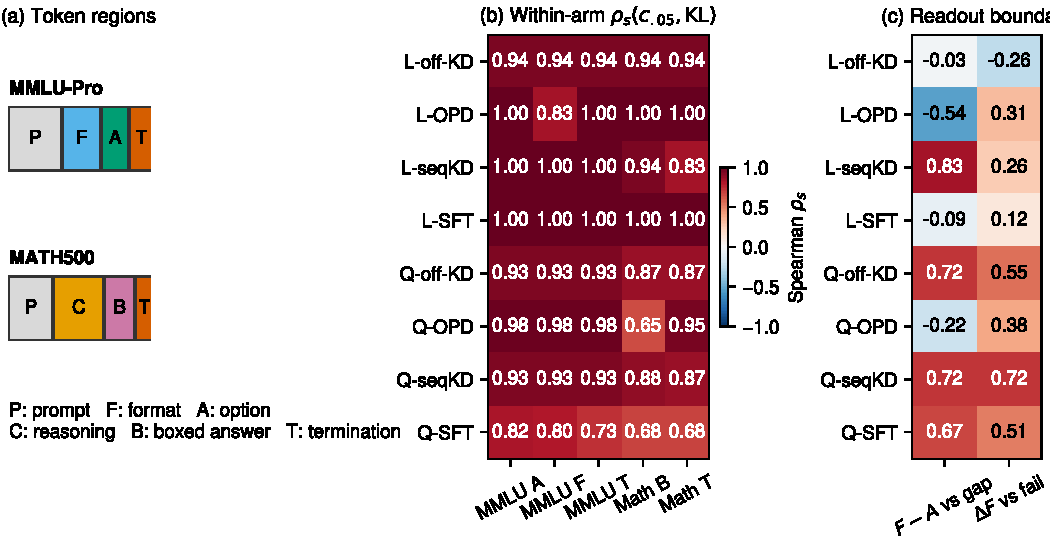
\includegraphics[width=\textwidth]{figures/fig3_regional_output.pdf}
\caption{区域输出关系。（a）每个模型和训练设置内，equal-5 功能压缩与区域 full-vocabulary KL 的跨 checkpoint Spearman。MMLU-Pro 的列为格式 $F$、正确选项标签 $A$ 和终止 $T$；MATH500 的列为推理 $C$、boxed answer $B$ 和终止 $T$。（b）MMLU-Pro 格式--答案 signed-NLL contrast 与 strict--flexible gap，以及格式 NLL 与 extraction failure 的相关。L 和 Q 分别表示 Llama 与 Qwen；每格数值给出相关系数。}
\label{fig:regional}
\end{figure*}

\begin{table*}[!t]
\centering
\small
\setlength{\tabcolsep}{4pt}
\begin{tabular}{llcc}
\toprule
模型/域 & 区域 & Held-out $R^2$: $C_5$ & Best $P_{k,5}$ \\
\midrule
Llama / MMLU-Pro & $A/F/T$ & \textbf{.869/.932/.468} & .743/.788/.459 \\
Llama / MATH500 & $B/T$ & .561/\textbf{.812} & \textbf{.615}/.647 \\
Qwen / MMLU-Pro & $A/F/T$ & \textbf{.426/.577/.596} & .243/.318/.443 \\
Qwen / MATH500 & $B/T$ & \textbf{.227}/.604 & .167/\textbf{.718} \\
\bottomrule
\end{tabular}
\caption{区域 full-vocabulary KL 的样本外预测。$C_5$ 与 $P_{k,5}$ 使用相同五模块、共同状态和 checkpoint-held-out folds。数值按区域顺序排列；粗体为逐区域更高的 $R^2$。后补 Math $C$ 的轨迹内和 checkpoint-demeaned 结果在正文报告，其 matched held-out 横向比较不在本表中。}
\label{tab:regional-prediction}
\end{table*}


\subsection{功能谱提供纯激活与纯权重坐标之外的轨迹信息}

图~\ref{fig:main} 将相同训练设置和 checkpoint 上的四种观察量并列。ER 记录激活协方差的谱维数；TPNT 记录更新坐标在 source principal mask 上的富集；PABS 记录主权重子空间的旋转；功能谱则记录当前权重在域上实际访问方向中形成的输出模式。前三者不能通过纵轴幅度与功能谱直接比较，但可以比较它们是否产生一致的训练轨迹结构。

纯激活轨迹没有复现功能谱的分离。Llama 多个外部域中，OPD@160 的 ER 相对变化不足 $.003$，step-0 CKA 仍约为 $.9997$--$1.0000$，而相同位置的 $r_{.05}$ 已减少约 14--26 个方向。TPNT 在部分 checkpoint 出现高于 spectrum-matched null 的局部富集，但未形成跨模型稳定的 OPD 特异轨迹；PABS 始终接近 1，配套 NSS 也很小，说明当前 LoRA 轨迹主要在近乎固定的主权重基底内演化。相较之下，图~\ref{fig:main} 最后一列中的 equal-5 功能压缩呈现清楚的训练设置分离。该差异来自 $W_t$ 与域输入度量的共同作用，而非更多同类特征。完整原生指标、null 与层级结果见 Supplementary Secs.~B.4 与 C.3。

在两个模型各 64 个严格共同状态上，我们进一步按 checkpoint group 留出训练阶段。完整 activation suite $A$、功能压缩 $C_5$ 与 source-principal block $P_{k,5}$ 的 OPD 识别结果见表~\ref{tab:identification}。$C_5$ 在两模型中都提供更清楚的排序判别；在三个输出目标的同协议比较中，它也均优于 raw activation block。strict $p_k$ 仍保留 Qwen absolute-NLL 的局部优势，说明功能状态与权重位置提供任务依赖的互补信息，而非普遍支配关系（Supplementary Sec.~D.3）。

\subsection{OPD 支配共同早期功能压缩}

图~\ref{fig:main} 最后一列显示，两种模型中的 OPD 都在共同早期窗口进入更深的功能压缩状态。为检验域平均是否掩盖排序反转，定义 OPD 相对最接近离线设置的边际
\begin{equation}
M_{m,D,t}
=\min_{b\in\{\mathrm{SFT,offKD,seqKD}\}}\Delta r_{m,b,D,t}^{(5)}
-\Delta r_{m,\mathrm{OPD},D,t}^{(5)}.
\end{equation}
$M>0$ 表示 OPD 比每个离线设置都更压缩。在 $\varepsilon=.05$ 下，两模型四域和 step 20/40/80 的最小边际均为正；完整逐域曲线见 Supplementary Sec.~C.1。为概括完整轨迹，我们再在 $\tau=\log(1+t)$ 上积分基线以下压缩至 $T=320$，得到 negative contraction dose（NCD）。表~\ref{tab:ncd} 分别保留早期排序和全程剂量：OPD 在两模型中都具有最大 NCD。

四个阈值、连续谱、centered covariance 与层级审计保持这一结论；逐模块结果表明 OPD 最深的排序在 value/output 与 MLP 中更稳定，而 q/k 具有异质性。它不表示压缩能量只来自五类模块。完整 equal-7、层级和模块结果见 Supplementary Secs.~C.2--C.3。

\subsection{Exposure 与 Refresh 组织轨迹，但不决定读出}

在相同 forward-KL 下，Qwen 的 $\alpha=.5$ 轨迹沿 off-KD 到 OPD 有序移动，但并非严格一维插值（图~\ref{fig:controls}a）。Llama frozenSelf0-KD 则只移除 current-student rollout 的持续刷新。OPD 相对 frozenSelf0-KD 的压缩优势在五个固定外部域和全部后续 checkpoint 上持续存在（图~\ref{fig:controls}b--c），因此 current-support refresh bundle 是更直接的组织因素。由于 refresh 同时改变 rollout 长度、EOS、重复与风格，该对照识别的是总体 refresh bundle，而不是纯粹的 freshness 效应。

off-KD 与 seqKD 使用完全相同的 teacher sequences、顺序、步数和 LoRA 配置，只改变监督目标。表~\ref{tab:support-readout}A 显示，二者在 Qwen 四个核心域中形成高度一致的功能路径；Llama 的模式预算总体接近，但 General 域的时间同动具有异质性。行为读出并未被这些路径锁定：Qwen 的 seqKD 在终点出现显著更高的 MATH500 cap-hit，并伴随 accuracy 和格式读出的变化，而 Llama 没有复现同等幅度的分叉（表~\ref{tab:support-readout}B）。相同 sequence support 可以组织相近的功能模式预算，target distribution 仍能改变具体读出。

\subsection{相对功能压缩追踪区域无符号输出移动}

图~\ref{fig:regional}a 比较 $c_{.05}^{(5)}$ 与区域 KL 在每条训练设置内的相关。MMLU 的格式、答案和终止，以及 MATH 的推理、boxed answer 和终止，大多数都随功能压缩同步移动；Math CoT 区域在两个模型的四种设置中也全部为正。为固定训练阶段，我们在每个 model--domain--checkpoint 内减去同期四设置均值。Math $\mathrm{KL}_C$ 的相关在 Llama/Qwen 中仍为 $.875/.573$，而 $\mathrm{KL}_B$ 为 $.902/.440$；regional contrast $\mathrm{KL}_B-\mathrm{KL}_C$ 则为 $-.209/-.183$。因此功能压缩追踪各区域移动了多少，却不决定移动主要分配到推理还是最终答案。

表~\ref{tab:regional-prediction}进一步在原先冻结的实际 KL 区域上比较 $C_5$ 与强权重基线 $P_{k,5}$。功能谱在大多数区域取得更高样本外 $R^2$，明确例外是 Llama Math boxed-answer 与 Qwen Math termination。该横向比较尚不包含后补的 Math $C$，因而不把新区域并入旧胜负汇总。扩展到 signed 与 absolute targets 后，两个坐标的平均差距缩小；完整固定参考序列合并为单一区域时，无符号关系仍然存在（Supplementary Secs.~D.1--D.3）。

\subsection{Signed Readout 与真实行为具有模型依赖性}

KL 测量移动幅度；signed NLL 进一步询问 reference token 变得更容易还是更困难。MMLU-Pro 的 $\Delta\mathrm{NLL}_{F-A}$ 对比格式与答案区域，MATH 的 $\Delta\mathrm{NLL}_{B-C}$ 对比 boxed answer 与之前推理。它们到 strict--flexible gap 或 extraction failure 的关系在模型和训练设置之间改变符号（图~\ref{fig:regional}b）。例如，$F-A$ 在 Qwen off-KD/seqKD 中与格式缺口正相关，却在 Qwen OPD 和 Llama OPD 中负相关。功能模式数量、区域分配、reference-token 读出效价和自由生成行为因而是相关但不可合并的层次。

这一边界与 matched-support 结果一致。功能谱可以描述 sequence support 如何组织局部模式预算，以及输出分布移动了多少，但单一 rank 不能判断这些移动改善还是损伤任务。Qwen adapter zeroing 和答案位概率质量审计进一步支持格式/readout 通道解释，但属于模型特定的补充证据（Supplementary Sec.~D.5）。


\section{讨论}

域条件功能谱的价值不在于取代裸权重或输出评测，而在于提供模式分离的中间观察。裸权重坐标告诉我们更新写入 source 参数结构的哪里，行为 Eval 告诉我们完整网络最终是否完成任务；$W_tS_{D,t}$ 则把当前权重映射到输入域实际访问的白化坐标，使每个奇异模式具有直接的本层输出能量含义。它因此能区分“参数位置接近但功能预算不同”和“功能预算接近但读出不同”的情形。

功能压缩也不等于能力被删除。它表示主要本层输出能量集中到更少模式；这些模式可能更有效，也可能把概率质量导向不合适的推理、格式或终止通道。区域 KL 进一步表明，模式数量、区域分配、读出效价和序列级任务实现不能被压成同一轴。

\section{局限性}

每个模型、每种训练设置目前只有一条独立 LoRA 轨迹，跨 checkpoint 和 domain 的一致性不能替代独立 seeds。双模型严格网格也只有四个 held-out checkpoint groups，AUC 表示排序而非概率校准。该理论对固定模块的线性二阶输出误差精确，但不包含残差路径、后续非线性和最终 token readout；其行为联系因此是经验关联而非端到端因果归因。centered、连续谱和完整模块审计目前在 Llama 上最完整，frozen-self 也只在 Llama 上完成。最后，current refresh 的总效应已经被更直接地识别，但长度、EOS、重复和风格等中介尚未进一步拆分。

\section{结论}

本文把 activation-aware 低秩空间转化为逐 checkpoint 的后训练观察方法。域条件功能谱将当前权重置于输入域实际访问的白化坐标中，使奇异谱直接对应本层输出能量，并保留精确的最优低秩误差解释。

在 Qwen 与 Llama 上，该空间区分出不同训练轨迹并揭示 OPD 的共同早期功能压缩；exposure 与 frozen-self 对照进一步指向 current-support refresh 的组织作用。相对压缩追踪推理、格式、答案和终止区域的无符号输出移动，而区域分配、matched-support 与 signed readout 结果说明功能模式预算和最终行为可以分离。这个中间观察层由此连接了训练 support、模块功能重组和模型输出，同时保留了权重分析与行为评测各自不可替代的作用。

\bibliography{references}

\end{CJK*}
\end{document}
